This chapter presents a detailed explanation of the neural network models proposed in this work and
the correspondent baselines used for comparison. In section one the architectures of
the main networks are shown. In section 2 the loss functions used are described. Finally,
section 3 shows the baselines models used for the ablation study of both performance and
explainability.

\section{Network architectures}
As was mentioned before, the main principle followed for model design is to enhance explainability
while maintaining performance as much as possible. With that in mind, we combine two
state of the art techniques from the deep learning literature, semantic segmentation
and attention mechanisms to design three novel architectures that present a significant
improvement in explainability over traditional blackbox CNNs. We describe these architectures
in the following sub sections, ordered by model complexity. Is important to note that
for learning to rank on placepulse
2 forward passes of ranking the network are required for each data instance (one for each image) and both scores are used
for calculation of the loss. See section \ref{section:loss} for  details.


\subsection{Segmentation as a feature extractor.}
The traditional deep learning approach in computer vision, consists of using a pretrained
CNN \cite{lecun_mnist}, on the Imagenet dataset \cite{imagenet}, such as the ResNet \cite{he_resnet},
usually called the feature extractor, and then stacking a custom set of layers over its output features. Leaving the CNN weights
fixed or updating them on training  depends on the particular problem. This is the approach taken
by most of the previous literature on urban perception \cite{hidalgo_placepulse,tamara_judgments,zhang_measuring}.

In this work, we propose replacing the traditional feature extractors for a fully trained semantic segmentation
network. The semantic segmentation task consists of assigning a label to every pixel in an image, and therefore
it implies a fine grained detection of object edges, providing a rich amount of information that is human understandable.
The output of a semantic segmentation model is a probability distribution over the different classes for each pixel,
making it usable as a feature map of the image. See figure \ref{fig:segmentation} for an example.

We base our models on the PSPNet architecture \cite{pspnet}, since it is one of the highest performing models
available in the literature. It's design its based on a ResNet50 and a pyramid pooling module, which consists on
parallel poolings and convolutions at different scales, that are then concatenated and used to generate the output with a
final convolution.

\begin{figure}[ht]
	\begin{center}
	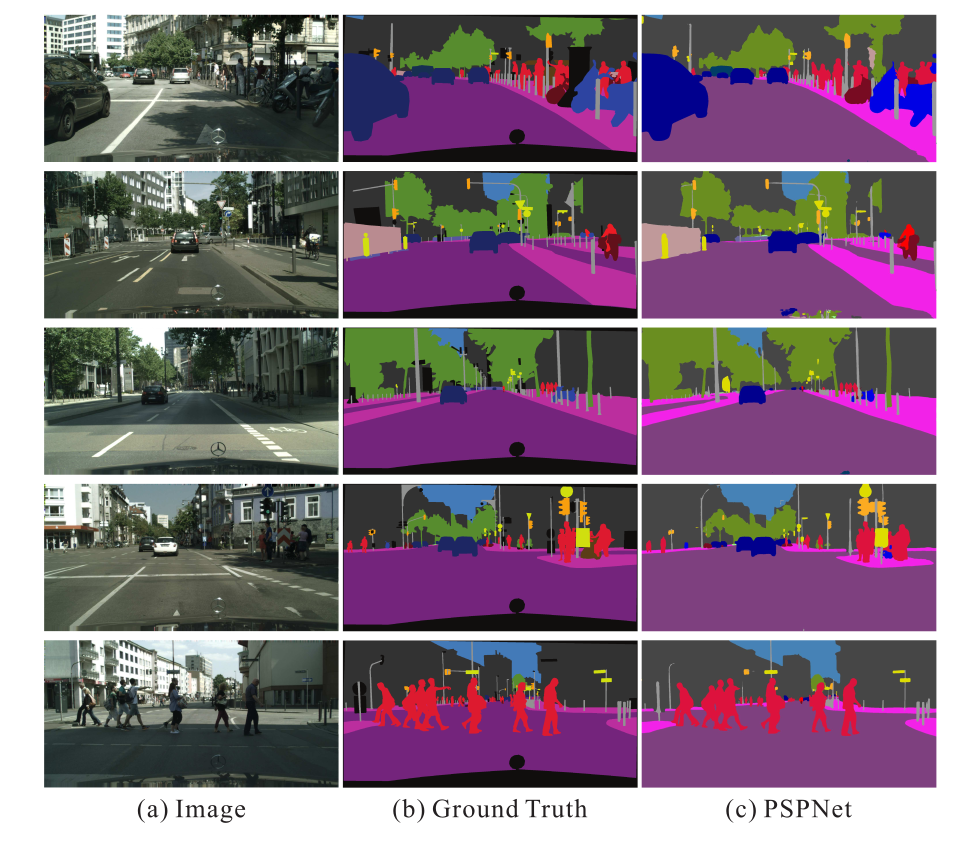
\includegraphics[width=0.8\textwidth]{./figures/segmentation.png}
	\caption[Example of Semantic Segmentation]{Examples of semantic segmentation by the PSPNet model on the CityScapes dataset. Extracted from \citeA{pspnet} }
	\label{fig:segmentation}
	\end{center}
\end{figure}

\begin{figure}[ht]
	\begin{center}
	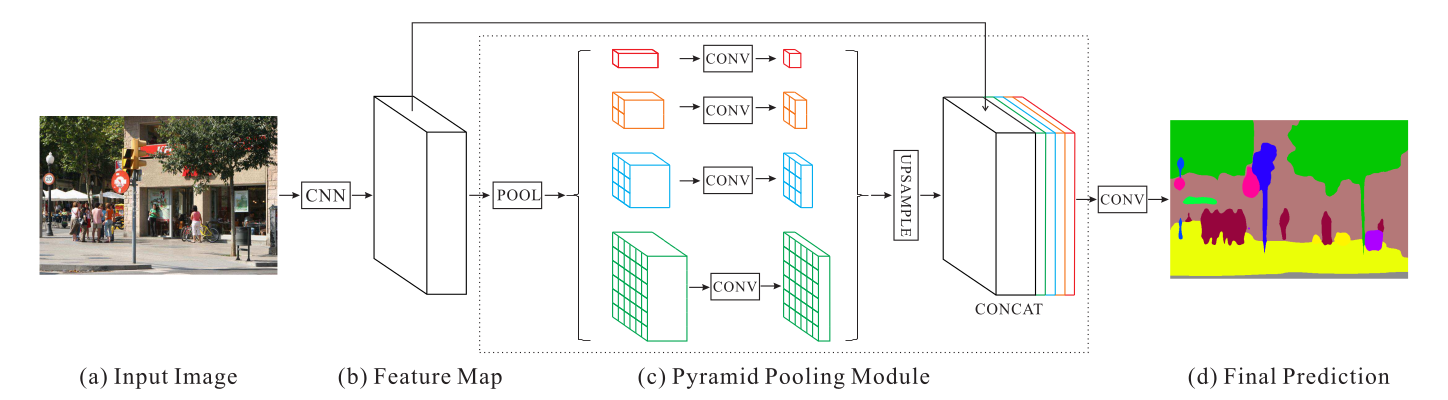
\includegraphics[width=0.9\textwidth]{./figures/pspnet.png}
	\caption[PspNet architecture]{PSPNet architecture. Extracted from \citeA{pspnet} }
	\label{fig:segmentation}
	\end{center}
\end{figure}

We train PspNet on the CityScapes dataset \cite{cordts_cityscapes}, since its urban images taken from a car have
considerable similarity to street view images, and its classes have proven informative for the urban perception problem
in previous research \cite{rossetti,zhang_measuring}. After this process we keep the network weights fixed
and use the output as features for subsequent layers. The segmentation output  is a tensor $S$, $S \in \mathbb{R}^{h\times w \times C}$, with $C$
the number of different classes. We experiment with using the features directly or applying a softmax operation.

For the calculation of the ranking score, we apply a linear transformation to every pixel distribution, flattening the output to
$\mathbb{R}^{h \times w}$  and then an MLP with one hidden layer and ReLU activation. The final linear layer
of the MLP generates a single scalar value representing the perception score.

\begin{figure}[ht]
	\begin{center}
	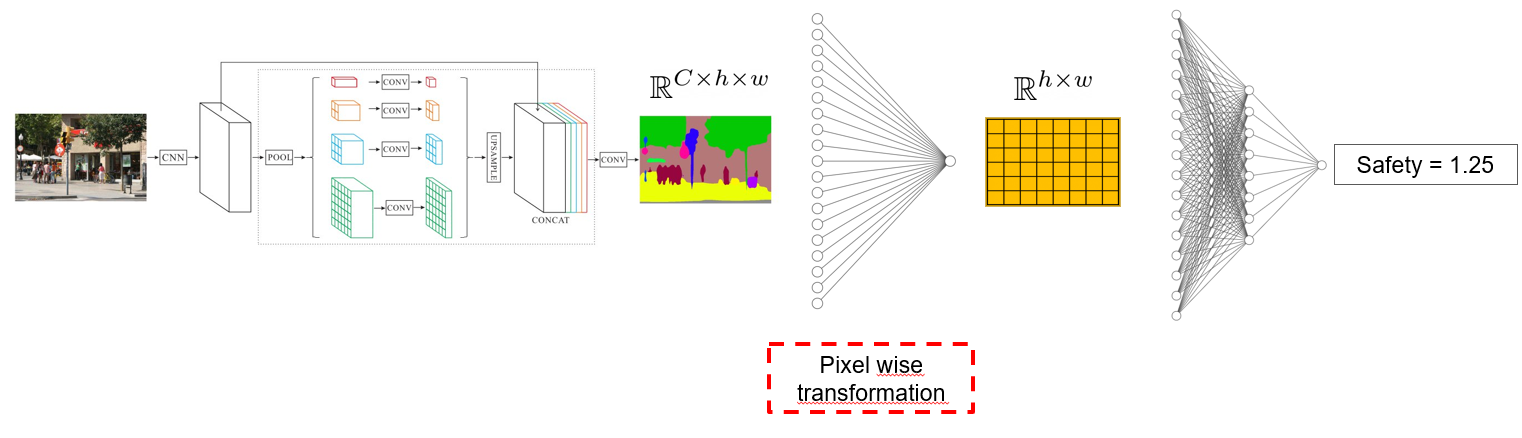
\includegraphics[width=0.9\textwidth]{./figures/segrank_1.png}
	\caption[First model architecture]{First model architecture}
	\label{fig:segrank_1}
	\end{center}
\end{figure}

\subsection{Self attention.}
With the intention of improving performance and explainability of the model, we process
the segmentation output with self attention mechanisms instead of a traditional MLP as
they have been proven to provide both benefits by previous research \cite{vaswani_attention, wiegreffe_attention, cordonnier_relationship}.

For our model we use a simplified version of the multihead attention mechanism
proposed by \citeA{vaswani_attention}, that consists of the same operations but
without splitting the input in several heads. We do this because using multiple heads
reduces the interpretability of the attention outputs, since different heads may output
inconsistent weights, as is mentioned in \citeA{clark_bertlook} and \citeA{li_disagreement} and
also verified on this task by our own experiments.

The attention mechanisms receives three matrixes as input: the query $Q$, the key $K$ and the value
$V$. It calculates a matrix of attention weights over $V$ based on $Q$ and $K$ and the final output
is given by the product between $V$ and the weights. A linear transformation is defined
for each of the inputs with weights $W_Q, W_K, W_V$ respectively, and another transformation $W$
is applied to the final output. Formally the attention layer can be defined as:
\begin{align}
	\text{Attention}(Q,K,V) &= \text{softmax}(\frac{QK^T}{\sqrt{d_k}})V \\
	\text{AttentionLayer}(Q,K,V) &=  \text{Attention}(QW_Q,KW_K,VW_V)\cdot W
\end{align}
Where $d_k$ is the embedding size of the key. For the particular case of self attention,
the same input is used as query, key and value, so for our case we make $Q=K=V=S'$ with
$S' \in \mathbb{R}^{(hw) \times C}$ and equal to the segmentation output flattened to one
spatial dimension.




\subsection{Segmentation as attention query.}

\section{Loss function} \label{section:loss}
The loss function for this task must account for the pairwise structure of the dataset,
and should represent the cost of breaking restrictions given by equations
\ref{eq:constraints} and \ref{eq:constraints_ties}. For \ref{eq:constraints} we use
a hinge loss similar to the one proposed by \citeA{hidalgo_placepulse}:

\begin{equation}
	L_r(x_i,x_j,y | \Theta) = \max(0, -y(f_\Theta(x_i) - f_\Theta(x_j)) + m_r)
	\label{eq:r_loss}
\end{equation}

Where $f_\Theta$ and $\Theta$  represent the network and its parameters respectively, and $m_r$
is an hyperparameter. This loss component makes it so that the model learns to assign a higher
score to the image winner of the vote. Based on the work by \citeA{doughty_loss} we also add a second component so that tied votes can
be used for training. According with equation \ref{eq:constraints_ties} we define:

\begin{equation}
	L_t(x_i,x_j | \Theta) = \max(0, |f_\Theta(x_i) - f_\Theta(x_j)| - m_t)
	\label{eq:t_loss}
\end{equation}

Where $m_t$ is also an hyperparameter. Finally, the complete loss function is defined as:

\begin{equation}
	L(x_i,x_j,y | \Theta) =\left\{\begin{matrix}
		L_r(x_i,x_j,y)&\text{ if } y \in \{-1,1\} \\
		L_t(x_i,x_j)&\text{ if } y=0
	\end{matrix}\right.
\end{equation}

In practice we take the mean loss over the batch examples and we set $m_r=m_t=1$

\section{Baselines}

\subsection{ResNet50 + MLP}

\subsection{ResNet50 + Attention layer + MLP}